\documentclass{standalone}
\usepackage{tikz}
\begin{document}
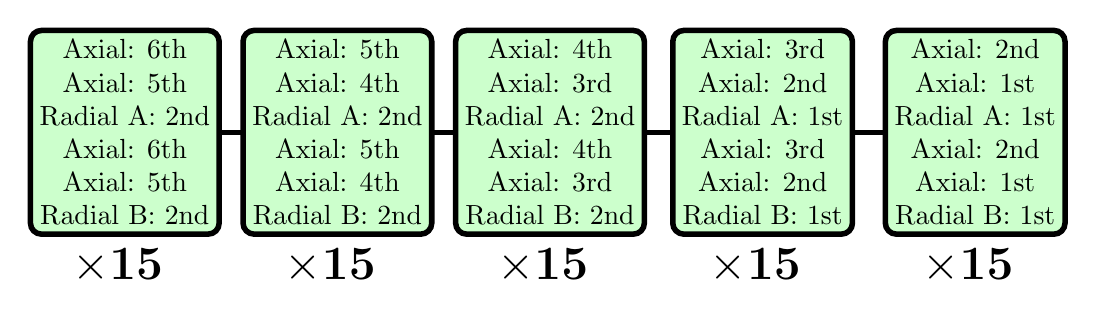
\begin{tikzpicture}
  \draw[line width=2] (0, 0) node[fill=green!20,draw,rounded corners,align=center]
  {
    Axial: $6$th\\
    Axial: $5$th\\
    Radial A: $2$nd\\
    Axial: $6$th\\
    Axial: $5$th\\
    Radial B: $2$nd} --
  ++(2.7, 0) node[fill=green!20,draw,rounded corners,align=center]
  {
    Axial: $5$th\\
    Axial: $4$th\\
    Radial A: $2$nd\\
    Axial: $5$th\\
    Axial: $4$th\\
    Radial B: $2$nd} --
  ++(2.7, 0) node[fill=green!20,draw,rounded corners,align=center]
  {
    Axial: $4$th\\
    Axial: $3$rd\\
    Radial A: $2$nd\\
    Axial: $4$th\\
    Axial: $3$rd\\
    Radial B: $2$nd} --
  ++(2.7, 0) node[fill=green!20,draw,rounded corners,align=center]
  {
    Axial: $3$rd\\
    Axial: $2$nd\\
    Radial A: $1$st\\
    Axial: $3$rd\\
    Axial: $2$nd\\
    Radial B: $1$st} --
  ++(2.7, 0) node[fill=green!20,draw,rounded corners,align=center]
  {
    Axial: $2$nd\\
    Axial: $1$st\\
    Radial A: $1$st\\
    Axial: $2$nd\\
    Axial: $1$st\\
    Radial B: $1$st
  };
  \path (0, -1.7) node[rounded corners,align=center]
  {
    \LARGE $\mathbf{\times 15}$
  } --
  ++(2.7, 0) node[rounded corners,align=center]
  {
    \LARGE $\mathbf{\times 15}$
  } --
  ++(2.7, 0) node[rounded corners,align=center]
  {
    \LARGE $\mathbf{\times 15}$
  } --
  ++(2.7, 0) node[rounded corners,align=center]
  {
    \LARGE $\mathbf{\times 15}$
  } --
  ++(2.7, 0) node[rounded corners,align=center]
  {
    \LARGE $\mathbf{\times 15}$
  };
\end{tikzpicture}
\end{document}
